\chapter{Literature Study}
\label{sec:lit}

The literature study introduces the reader to a few fundamental concepts, and similar implementations to give context to the project. It also briefly evaluates cost effectiveness.\\

Infrared light begins at the `red edge' of the visible spectrum from 700 nanometers (430 THz) to 1 mm (300 GHz) \cite{ir_wiki}. Due to the silicon response, the image sensor in consumer cameras can capture infra-red light up to 1000 nanometers \cite{ir_wiki} as in Figure \ref{fig:ir_spectrum} (excluding ultraviolet light). Also, there is a certain phenomenon which occurs within this region. Chlorophyll becomes transparent, and allows each vegetation cell to act as an elementary corner reflector. This accounts for a rapid change in reflectance, depending on the health of the plant, and is utilized in vegetation indices, such as the NDVI \cite{red_edge}.

\begin{figure}[H]
\centering
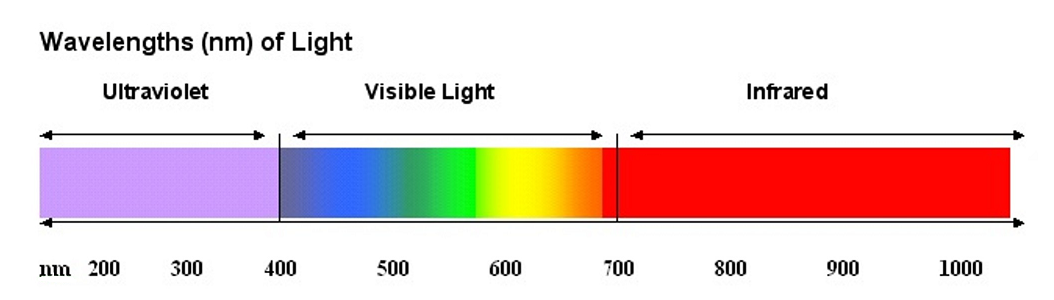
\includegraphics[scale=0.35]{images/ir_spectrum.png}
\caption{Wavelengths of light \cite{ir_spectrum}}
\label{fig:ir_spectrum}
\end{figure}


The normalized difference vegetation index (NDVI), is a useful visual indicator for analyzing remote sensing measurements, typical from a space platform\footnote{Aerial footage will always be higher resolution, with each pixel capturing under a few $cm^2$ as opposed to under a few $m^2$, and is useful for more in-depth analysis} More specifically, one can quantify whether the target being observed contains active green vegetation or not\cite{ndvi_wiki} as in Figure \ref{fig:ndvi_british}. The higher the values are, the more photosynthetically active the plants are, and in the following two pictures, the colour map ranges from black ($-1.0$) to dark green ($1.0$).

\begin{figure}[H]
\begin{subfigure}{0.5\textwidth}
\centering
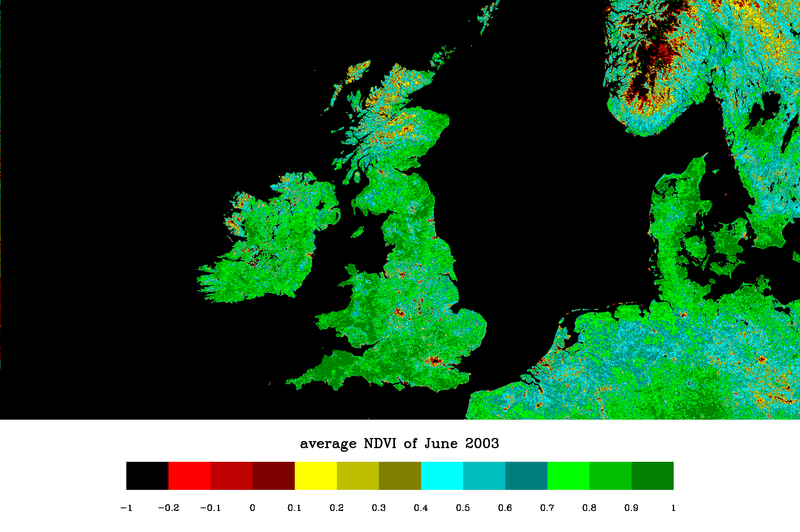
\includegraphics[scale=0.25]{images/NDVI_062003.png}
\caption{Summer in June 2003}
\end{subfigure}
\begin{subfigure}{0.5\textwidth}
\centering
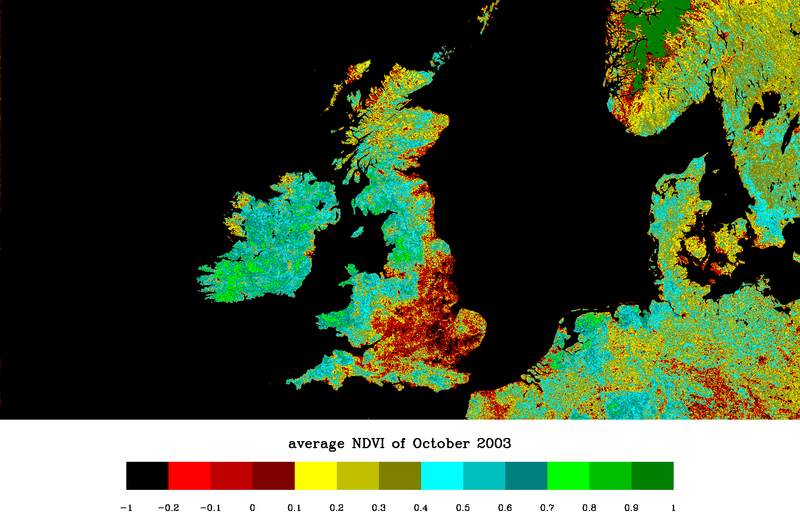
\includegraphics[scale=0.25]{images/NDVI_102003.png}
\caption{Autumn in October 2003}
\end{subfigure}
\caption{Average NDVI over the British Isles \cite{ndvi_wiki}}
\label{fig:ndvi_british}
\end{figure}

The NDVI is calculated using the following formula for each pixel:

\begin{equation}\label{eq:ndvi}
{\displaystyle{\mbox{NDVI}}={\frac {({\mbox{NIR}}-{\mbox{Red}})}{({\mbox{NIR}}+{\mbox{Red}})}}}, \in [-1.0, 1.0]
\end{equation}

where $RED$ and $NIR$ is the spectral reflectances\footnote{Fraction of incident electromagnetic power reflected at an interface} acquired in the red (visible) and near-infrared regions. The $RED$ band exists between 600 - 700 nm, and the $NIR$ band from 700 - 1000 nm. The `red-edge` band exists between 680 - 730 nm, and refers to the region of rapid change in reflectance of vegetation.

\begin{figure}[H]
\centering
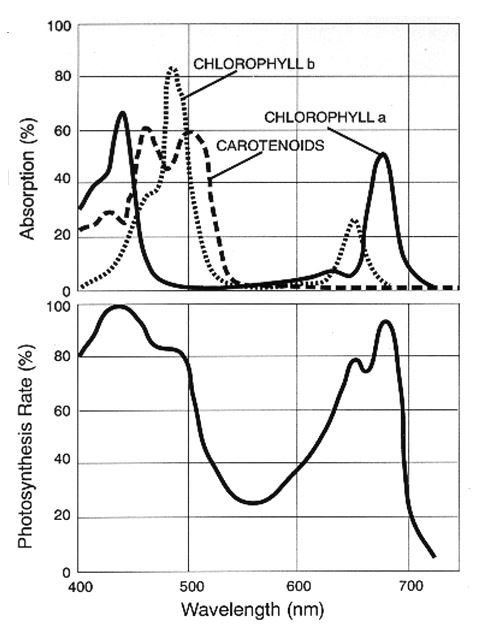
\includegraphics[scale=0.5]{images/chlorophyll.jpg}
\centering
\caption{Photosynthesis and absorption rate of plants \cite{ndvi_wiki}}
\label{fig:chlorophyll}
\end{figure}

Plants absorb mostly red (600 - 700 nm) and blue (400 - 500 nm) light. They absorb less green (500 - 600 nm) light. And they do not absorb light past 700 nm. The photosynthetically active radiation (PAR) region denotes this range (400 - 700 nm) where plants absorb light and photosynthesise.

In Figure \ref{fig:chlorophyll}, typical photosynthetic action in the (PAR) spectral region for live green plants is shown, beside absorption spectra for chlorophyll\footnote{Green pigment that absorbs light in blue and red bands.} and carotenoids\footnote{Organic pigments that absorb light energy mostly in blue band.}. Solar radiation is absorbed within this region as a source of energy. \\

Leaf cells reflect solar radiation in the NIR band because the photon energy at wavelengths longer than 700 nm is not sizeable enough to synthesize organic molecules, even though it comprises approximately half of the total incoming solar energy.\\

The rationale behind the NDVI is that one can exploit the stark differences in plant reflectance to determine their spatial distribution. Free-standing water and soils exhibit low values. Glass windows, on the other hand, exhibit high NDVI values.\\

Looking briefly at a history of the NDVI, the launch of Sputnik 1 by the Soviet Union in 1957 sparked an interest in meteorological satellites to improve weather forecasting. The NDVI was introduced in the early seventies by the ERTS\footnote{Earth Resources Technology Satellite, or Landsat 1}, and remains popular today. \\

Today, for example, one can expect to pay about 1600 USD per fortnightly 0.5 m resolution photo from the Pléiades satellite constellation\footnote{Very-high-resolution optical earth-imaging satellites via Satellite Imaging Corporation}. There are other sensors with similar pricing, including the WorldView, GeoEye, Kompsat, Quickbird, Gaofen etc.\\Aerobotics, based in Cape Town have quite a cost effective solution, with weekly footage at 500 ZAR per month, however at a low resolution of 10m per pixel. They also charge 80 ZAR per hectare for drone surveys, and 20 ZAR per hectare\footnote{Worldwide average farm size is 59.4 Ha\cite{farm_size}, South Africa between 427 - 5799 Ha \cite{farm_size_sa}} if one uploads one's own data (they will process the data online). Solutions like these show that it could be beneficial for a farmer to have their very own automated solution.\\

One can argue that there has always been an effort to find more cost effective solutions to commercial applications, including NDVI analysis. If an inexperienced farmer were to perform NDVIs of their land by themselves, there does exist online platforms to process the imagery. However, imagery may not necessarily be calibrated, and distortions in the lens may create an inaccurate result. High upfront costs may be too much especially for smaller-scale farmers. Typical drones like the Phantom series cost around 1000-2000 USD. The Parrot Sequoia, which has 5 cameras, retails at 3500 USD \cite{sequoia}. The Mapir Survey2, which is a converted single camera solution, retails at 500 USD \cite{mapir}, and the AgroCam Pro, which has dual cameras, retails at 575 USD \cite{agrocam}.\\

Just to place the NDVI within a larger context, it is not the only vegetation index. One such example is the Enhanced vegetation index in Equation \ref{eq:evi},

\begin{equation}\label{eq:evi}
EVI=G\times {\frac  {(NIR-Red)}{(NIR+C1\times Red-C2\times Blue+L)}}
\end{equation}

where $NIR$, $Blue$ and $Red$ refer to atmospherically corrected Raleigh and ozone absorption surface reflectances, $L$ refers to background adjustment in canopies that address non-linear, differential $NIR$, and the coefficients $C1$, $C2$ uses the blue band to correct for aerosol influences in the $Red$ band. The EVI, as opposed to the more chlorophyll sensitive NDVI, is more responsive to structural canopy variations, including leaf index area and physiognomy\footnote{External appearance, and growth forms of dominant taxa} \cite{evi}. Since it has more of a satellite application, this exists outside the scope of the project.\\

Another example is the normalized difference water index as in Equation \ref{eq:ndwi},

\begin{equation}\label{eq:ndwi}
{\displaystyle {\mbox{NDWI}}={\frac {(NIR-SWIR)}{(NIR+SWIR)}}}\quad or\quad {\displaystyle {\mbox{NDWI}}={\frac {(Xgreen-NIR)}{(Xgreen+NIR)}}}
\end{equation}

with:
$Xgreen$ being light from the green channel from 500 - 600 nm.\\


where short-wave infrared SWIR\footnote{Water absorption increases significantly at 1450 nm, within SWIR wavelength 1.4-3 µm} wavelengths are used to monitor changes in water content of leaves, and green and NIR wavelengths monitor changes realted to water content in water bodies. The former is useful for vegetation, and the latter is useful to detect flooding or changes in water level \cite{ndwi}. SWIR cameras are expensive, however.\\

Back to NDVIs, it should be noted that there are many who motivate that a cheap conversion of a normal digital camera (by replacing the NIR filter with a blue or red filter) will show satisfactory results. Specialists would generally advise one to avoid such methods since one can never remove the cross-channel interference (see Section \ref{image_acq}), unless one has dual/stereo cameras. They also warn against several problems such as distortion, differences in focal length, rotation and translation between the cameras, and so forth.\\

There exist techniques to solve these problems, with an initial step to calibrate the cameras using corresponding points in a 3D plane \cite{calib3d}. Commonly, a set of chessboard images is used. Then, images are stereo-rectified \cite{calib3d} and undistorted \cite{calib3d}. The common area may still differ in focal length, and due to motion, and for this reason feature matching and homography is used to align the images as best as possible. Only then can an NDVI be calculated for each matching pixel on an image pair. In mapping, one can separately create an RGB and NIR map, and then use an image registration method to match the maps \cite{bunwarpj}.

